\subsection{Generating Sets and Cayley Digraphs}


%%%%%%%%%%%%%%%%%%%%%
%  Generating Sets  %
%%%%%%%%%%%%%%%%%%%%%

\subsubsection{Generating Sets}

So far, we have talked about cyclic groups, which are generated by a single element. But many groups require more than one generator. The idea extends naturally: given elements $a_1, a_2, \ldots \in G$, the subgroup generated by them consists of all finite products of their integer powers.

\Definition{Intersection of sets}{
    Let $\Set{S_i}{i \in I}$ be a collection of sets. Here, $I$ may be any set of indices. The \textbf{intersection} $\displaystyle \bigcap \limits_{i \in I}$ \textbf{of the sets} $S_i$ is the set of all elements that are in all the sets $S_i$. That is, \[ 
        \bigcap \limits_{i \in I} S_i = \Set{x}{\forall i \in I, x \in S_i}
    \]
    If $I$ is finite, $I = \{ 1,2,\dots,n \}$ we may denote $\bigcap \limits_{i \in I} S_i$ by \[ 
        S_1 \cap S_2 \cap \cdots \cap S_n
    \]
}

\Theorem{}{
    For any group $G$ and any nonempty collection of subgroups $\Set{H_i \leq G}{i \in I}$, the intersection of all the subgroups $H_i, \displaystyle \bigcap \limits_{i \in I} H_i$, is also a subgroup of $G$.
}

\Proof{
    We verify the conditions of the two-step test for $\bigcap \limits_{i \in I} H_i$:
    \begin{enumerate}
        \item \textbf{Closure:} Let $a, b \in \bigcap \limits_{i \in I} H_i$. Then $a, b \in H_i$ for every $i \in I$. Since each $H_i$ is a subgroup, $ab \in H_i$ for every $i$, so $ab \in \bigcap \limits_{i \in I} H_i$.
        \item \textbf{Inverses:} If $a \in \bigcap \limits_{i \in I} H_i$, then $a \in H_i$ for every $i$. Since each $H_i$ is a subgroup, $a^{-1} \in H_i$ for every $i$, so $a^{-1} \in \bigcap \limits_{i \in I} H_i$.
    \end{enumerate}
    Thus, $\bigcap \limits_{i \in I} H_i$ is a subgroup of $G$.
}

\Definition{Subgroup Generated by a Set}{
    Let $G$ be a group and let $\{a_i \mid i \in I\} \subseteq G$. The \textbf{subgroup generated by $\{a_i \mid i \in I\}$} is the smallest subgroup of $G$ containing all the $a_i$. If this subgroup equals $G$ itself, then $\{a_i \mid i \in I\}$ \textbf{generates} $G$, and the $a_i$ are called \textbf{generators of $G$}. A group is \textbf{finitely generated} if it has a finite generating set.
}

\Note{
    The ``smallest subgroup containing all the $a_i$'' exists because the intersection of any collection of subgroups is again a subgroup. So we can take the intersection of all subgroups of $G$ that contain all the $a_i$.
}

\Theorem{}{
    If $G$ is a group and $\{a_i \mid i \in I\}$ is a nonempty subset of $G$, then the subgroup $H$ generated by $\{a_i\}$ consists of precisely those elements of $G$ that can be written as finite products of integer powers of the $a_i$ (where powers of a fixed $a_i$ may occur multiple times in the product).
}

\Proof{
    Let $H$ be the subgroup generated by $\Set{a_i}{i \in I}$, which is the smallest subgroup of $G$ containing every $a_i$. Now, define the set: \[ 
        K = \Set{a_{i_1}^{n_1} \cdot a_{i_2}^{n_2} \cdots a_{i_k}^{n_k}}{k \in \Z^+, i_j \in I, n_j \in \Z} \cup \{e\}
    \]
    We want to show that $H = K$.

    \begin{itemize}
        \item \textbf{$K$ is a subgroup of $G$:} First, we verify that $K$ is a subgroup of $G$:
            \begin{enumerate}
                \item \textbf{Closure:} Let $x = a_{i_1}^{n_1} \cdots a_{i_k}^{n_k}$ and $y = a_{j_1}^{m_1} \cdots a_{j_l}^{m_l}$ be elements of $K$. \\
                    Then $xy = a_{i_1}^{n_1} \cdots a_{i_k}^{n_k} a_{j_1}^{m_1} \cdots a_{j_l}^{m_l}$, which is also an element of $K$ since it is a finite product of integer powers of the $a_i$.
                \item \textbf{Inverses:} Let $x = a_{i_1}^{n_1} \cdots a_{i_k}^{n_k}$ be an element of $K$. Then $x^{-1} = a_{i_k}^{-n_k} \cdots a_{i_1}^{-n_1}$, which is also an element of $K$ since it is a finite product of integer powers of the $a_i$.
            \end{enumerate}
            Thus, $K \leq G$.

            Each $a_i = a_i^1$ is a finite product of length $1$ with integer exponent, so \[ 
                \forall i \in I, a_i \in K
            \]
        \item \textbf{$K$ contains every $a_i$:} Each $a_i = a_i^1$ is a finite product of length $1$ with integer exponent, so $a_i \in K$ for every $i \in I$.
        \item \textbf{$H \subseteq K$:} Since $H$ is the smallest subgroup containing every $a_i$, and $K$ is a subgroup containing every $a_i$, we must have $H \subseteq K$.
        \item \textbf{$K \subseteq H$:} Since $H$ is a subgroup containing every $a_i$, it must contain every integer power of each $a_i$ (by closure and inverses). Since $H$ is closed under the group operation, it must contain every finite product of integer powers of the $a_i$. Thus, $K \subseteq H$.
    \end{itemize}
}

\Example{}{
    The dihedral group $D_n$ is generated by $\{\mu, \rho\}$: every element can be written as $\rho^k$ or $\mu\rho^k$ for $0 \leq k < n$. It is also generated by $\{\mu, \mu\rho\}$ since $\rho = \mu(\mu\rho)$. Interestingly, both $\mu$ and $\mu\rho$ have order 2, while in the set $\{\mu, \rho\}$, one generator has order 2 and the other has order $n$.
}

\Example{}{
    The Klein 4-group $V = \{e, a, b, c\}$ is generated by $\{a, b\}$ since $ab = c$. It is also generated by $\{a, c\}$ or $\{b, c\}$. Adding more elements to a generating set still generates the group: $\{a, b, c\}$ generates $V$ too.
}

\Example{}{
    The group $\Z_6$ is generated by $\{1\}$ (cyclic!) and by $\{5\}$. It is also generated by $\{2, 3\}$ since $2 + 3 = 5$, and $5$ generates $\Z_6$. However, $\{2, 4\}$ does \textit{not} generate $\Z_6$ since $\langle 2 \rangle = \{0, 2, 4\}$ and $\langle 4 \rangle = \{0, 4, 2\}$, so $\langle 2, 4 \rangle = \{0, 2, 4\}$ is a proper subgroup of $\Z_6$.
}


%%%%%%%%%%%%%%%%%%%%%
%  Cayley Digraphs  %
%%%%%%%%%%%%%%%%%%%%%

\subsubsection{Cayley Digraphs}

For each generating set $S$ of a finite group $G$, we can draw a \textbf{Cayley digraph} (directed graph) that visually represents the group structure:
\begin{itemize}
    \item One \textbf{vertex} (dot) for each element of $G$.
    \item For each generator $s \in S$, a type of \textbf{arc} (arrow). An arc of type $s$ from vertex $g$ to vertex $h$ means $gs = h$.
    \item If a generator $s$ satisfies $s^2 = e$ (it is its own inverse), we draw the arc without an arrowhead.
\end{itemize}

\Note[Properties of Cayley Digraphs]{
    Every Cayley digraph for a group satisfies:
    \begin{enumerate}
        \item \textbf{Connected:} We can get from any vertex to any other by traveling along arcs (because $gx = h$ always has a solution).
        \item \textbf{At most one arc from $g$ to $h$:} The solution of $gx = h$ is unique.
        \item \textbf{Regularity:} Each vertex has exactly one outgoing and one incoming arc of each type (for generator $b$, $gb$ is unique, and $xb = g$ has unique solution $x = gb^{-1}$).
        \item \textbf{Consistency:} If two different sequences of arc types starting from $g$ lead to $h$, then those same sequences starting from any vertex $u$ lead to the same vertex $v$.
    \end{enumerate}
    Conversely, any digraph satisfying these four properties is a Cayley digraph for some group.
}

\Example{Cayley digraph for $\Z_6$ with $S = \{1\}$}{
    With a single generator, we get a directed cycle through all elements:
    \begin{figure}[H]
        \centering
        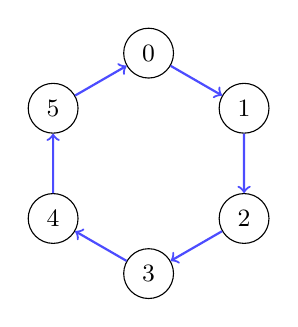
\begin{tikzpicture}[scale=1.4, every node/.style={font=\small}]
            \foreach \k in {0,...,5} {
                \pgfmathsetmacro{\angle}{90 - \k * 60}
                \node[circle, draw, fill=white, inner sep=2pt, minimum size=18pt] (n\k) at (\angle:1) {$\k$};
            }
            \foreach \k in {0,...,4} {
                \pgfmathtruncatemacro{\next}{\k + 1}
                \draw[->, thick, blue!70] (n\k) -- (n\next);
            }
            \draw[->, thick, blue!70] (n5) -- (n0);
        \end{tikzpicture}
        \caption{Cayley digraph for $\Z_6$, $S = \{1\}$}
    \end{figure}
}

\Example{Cayley digraph for $\Z_6$ with $S = \{2, 3\}$}{
    With two generators, we use solid arrows for $2$ and dashed (arrowless) edges for $3$ (since $3 + 3 = 0$ in $\Z_6$, so $3$ is its own inverse):
    \begin{figure}[H]
        \centering
        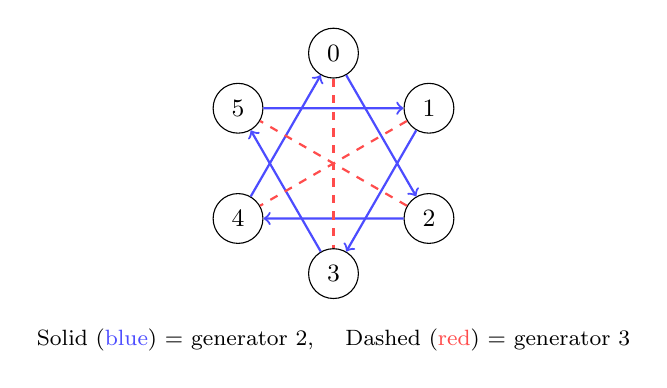
\begin{tikzpicture}[scale=1.4, every node/.style={font=\small}]
            \foreach \k in {0,...,5} {
                \pgfmathsetmacro{\angle}{90 - \k * 60}
                \node[circle, draw, fill=white, inner sep=2pt, minimum size=18pt] (n\k) at (\angle:1) {$\k$};
            }
            % Solid arrows for generator 2: 0->2, 2->4, 4->0, 1->3, 3->5, 5->1
            \draw[->, thick, blue!70] (n0) -- (n2);
            \draw[->, thick, blue!70] (n2) -- (n4);
            \draw[->, thick, blue!70] (n4) -- (n0);
            \draw[->, thick, blue!70] (n1) -- (n3);
            \draw[->, thick, blue!70] (n3) -- (n5);
            \draw[->, thick, blue!70] (n5) -- (n1);
            % Dashed edges (no arrows) for generator 3: 0--3, 1--4, 2--5
            \draw[thick, dashed, red!70] (n0) -- (n3);
            \draw[thick, dashed, red!70] (n1) -- (n4);
            \draw[thick, dashed, red!70] (n2) -- (n5);
            \node at (0, -1.6) {\footnotesize Solid (\textcolor{blue!70}{blue}) = generator 2, \quad Dashed (\textcolor{red!70}{red}) = generator 3};
        \end{tikzpicture}
        \caption{Cayley digraph for $\Z_6$, $S = \{2, 3\}$}
    \end{figure}
}

\Example{Cayley digraph for $D_4$ with $S = \{\rho, \mu\}$}{
    The dihedral group $D_4$ has 8 elements. Using $\rho$ (rotation by $\pi/2$) as solid arrows and $\mu$ (a reflection, order 2) as dashed edges:
    \begin{figure}[H]
        \centering
        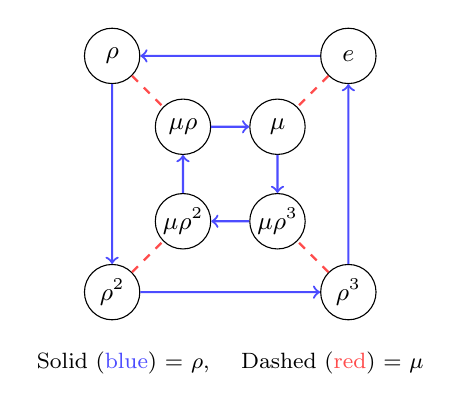
\begin{tikzpicture}[scale=1.5, every node/.style={font=\small}]
        % Outer square: rotations
            \node[circle, draw, fill=white, inner sep=1pt, minimum size=20pt] (e)  at (1, 1)   {$e$};
            \node[circle, draw, fill=white, inner sep=1pt, minimum size=20pt] (r)  at (-1, 1)  {$\rho$};
            \node[circle, draw, fill=white, inner sep=1pt, minimum size=20pt] (r2) at (-1, -1) {$\rho^2$};
            \node[circle, draw, fill=white, inner sep=1pt, minimum size=20pt] (r3) at (1, -1)  {$\rho^3$};
        % Inner square: reflections
            \node[circle, draw, fill=white, inner sep=1pt, minimum size=20pt] (m)   at (0.4, 0.4)   {$\mu$};
            \node[circle, draw, fill=white, inner sep=1pt, minimum size=20pt] (mr)  at (-0.4, 0.4)  {$\mu\rho$};
            \node[circle, draw, fill=white, inner sep=1pt, minimum size=20pt] (mr2) at (-0.4, -0.4) {$\mu\rho^2$};
            \node[circle, draw, fill=white, inner sep=1pt, minimum size=20pt] (mr3) at (0.4, -0.4)  {$\mu\rho^3$};
        % Solid arrows for rho (rotation)
            \draw[->, thick, blue!70] (e) -- (r);
            \draw[->, thick, blue!70] (r) -- (r2);
            \draw[->, thick, blue!70] (r2) -- (r3);
            \draw[->, thick, blue!70] (r3) -- (e);
            \draw[->, thick, blue!70] (m) -- (mr3);
            \draw[->, thick, blue!70] (mr3) -- (mr2);
            \draw[->, thick, blue!70] (mr2) -- (mr);
            \draw[->, thick, blue!70] (mr) -- (m);
        % Dashed lines for mu (reflection, order 2)
            \draw[thick, dashed, red!70] (e) -- (m);
            \draw[thick, dashed, red!70] (r) -- (mr);
            \draw[thick, dashed, red!70] (r2) -- (mr2);
            \draw[thick, dashed, red!70] (r3) -- (mr3);
            \node at (0, -1.6) {\footnotesize Solid (\textcolor{blue!70}{blue}) = $\rho$, \quad Dashed (\textcolor{red!70}{red}) = $\mu$};
        \end{tikzpicture}
        \caption{Cayley digraph for $D_4$, $S = \{\rho, \mu\}$};
    \end{figure}
}

\Note{
    From the Cayley digraph of $D_4$, we can read off products directly. For example, to compute $\mu\rho^2 \cdot \mu$: start at $\mu\rho^2$, follow a dashed edge to arrive at $\rho^2$. So $\mu\rho^2 \cdot \mu = \rho^2$.

    We can also detect whether a group is Abelian from its Cayley digraph: if for every pair of generators, following generator $a$ then $b$ from any vertex always gives the same result as following $b$ then $a$, the group is Abelian. For $D_4$, this fails: from $e$, $\rho$ then $\mu$ gives $\mu\rho^3$, but $\mu$ then $\rho$ gives $\mu\rho$.
}

\Note{
    A Cayley digraph makes the group's structure visible. The outer cycle in the $D_4$ diagram shows the cyclic subgroup of rotations $\langle \rho \rangle$, and the dashed edges connect each rotation to its corresponding reflection. The fact that the inner cycle runs in the \textit{opposite} direction reflects the relation $\rho\mu = \mu\rho^{-1}$.
}
